El diseño de la Kwii Platform vela por seguridad de la información de sus usuarios, es decir, las decisiones arquitecturales de la plataforma tuvieron en cuenta aspectos del menejo de la información de los usuarios con el fin de proveer al acceso a esta de manera fácil y eficaz, pero solo a los usuarios autorizados a obtenerla y además, las decisiones facilitan negar el acceso a esta información de manera rotunda a quien no esté autorizado. Es por ello que se plantea esta sección, donde se discutirán diferentes decisiones que fueron tomadas para hacer a la Kwii Platform un sistema seguro.
\subsection{Uso de un Servidor de Proxy Inverso}
En la arquitectura de la Kwii Platform, se plantean diferentes componentes que son encargados de numerosas responsabilidades dentro de la plataforma. Dichos componentes satisfacen las responsabilidades a las que son encargadas de maneras muy diversad pero, en general, para cumplir dichas responsabilidades los componentes exponen servicios que son consumidos por un único componente central que hace las de mediador en la arquitectura. Para evitar el acceso no autorizado con posibles acciones malintencionadas y garantizar que los servicios que prestan estos componentes sean únicamente consumidos por el componente central (tal y como lo plantea la vista de capas), se propone el uso de un Servidor de Proxy Inverso.
\\\\
\subsubsection{Justificación del uso de un Servidor de Proxy Inverso}
El Servidor de Proxy Inverso es el encargado de exponer los servicios compuestos del componente central, de exponer el componente Front End Web y de evitar el contacto de los demás componentes con el exterior exterior. La comunicación del mundo exterior con la Kwii Platform es representada en la siguiente figura:
\begin{center}
    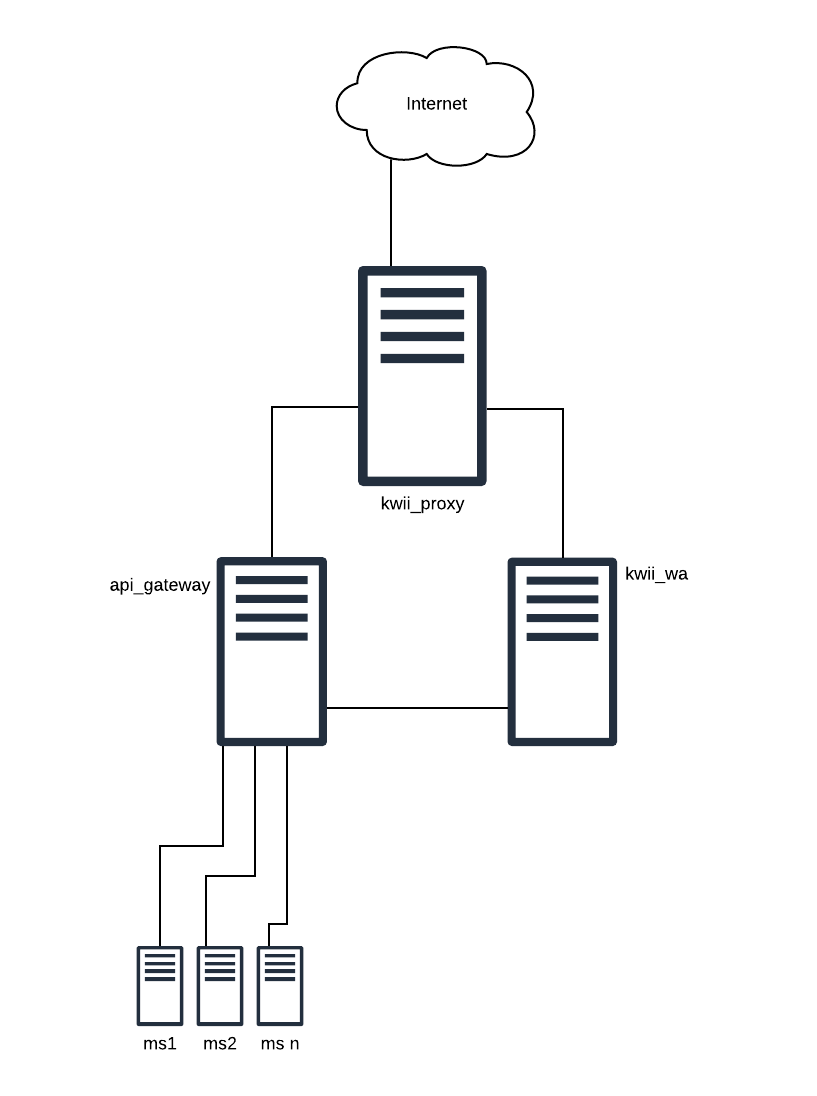
\includegraphics[width=8cm]{Figures/P4/InverseProxyDiagram1.png}
\end{center}
Como se mencionó anteriormente, cualquier intento de comunicación de otro elemento de la plataforma con el exterior será descartado.
\begin{center}
    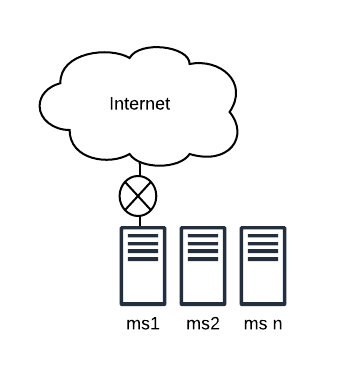
\includegraphics[width=5cm]{Figures/P4/InverseProxyDiagram2.png}
\end{center}
\subsubsection{Características de Seguridad Protegidas}
Las características de seguridad protegidos en la Kwii Platform a la hora de implementar un servidor de proxy inverson son las siguientes:
\begin{itemize}
    \item Confidencialidad\\\
    El servidor de proxy inverso potencia la confidencialidad de la información al disminuir los puntos de acceso a esta. Ahora, viéndonos limitados a acceder a la información de los demás componentes de la plataforma únicamente por medio del componente central, la arquitectura puede ser reforzada en estos aspectos únicamente tratando los flujos de información que pasan por dicho componente.
    \item Integridad\\\
    Así mismo como el servidor de proxy inverso asegura la confidencialidad, asegura también la integridad. Restringimos la cantidad de puntos de manipulación de la información.
    \item Disponibilidad
    Como trabajo futuro, el servidor de proxy inverso implementa dfunciones de balanceo de carga que garantizan la disponibilidad. (Próximamente)
\end{itemize}

\subsection{Manejo de Sesión de Usuarios}

Para el manejo de sesión de usuarios, la arquitectura de la Kwii Platform propone el uso de un esquema basado en tokens. En él, cualquier comunicación, solicitud de información, y en general, cualquier operación en la plataforma tiene que ser autorizada, por medio de la validación de tokens de usuario.

\subsubsection{Justificación del uso de autenticación basada en tokens}

Hay diversas características que hacen que la autenticación por tokens funcione bastante bien con la arquitectura propuesta de la Kwii Platform, entre ellas, se destacan las siguientes:

\begin{itemize}
    \item Los tokens siguen el principio stateless de la comunicación HTTP\\\
    Al contener en sí mismo la información de la sesión, los tokens nos permiten manipular la autenticación de los usuarios sin la necesidad de trazar su estado.
    \item Generación y manipulación centralizado\\\
    La arquitectura de nuestra aplicación permite que la autenticación sea manejada únicamente por los componentes encargados de ello, así los tokens son manipuladas de manera centralizada y el resto de los componentes que sean agregados a la arquitectura no se tienen que responsabilizar por cuestiones de autenticación.
    \item Control de acceso\\\
    El uso de tokens de usuario nos permite determinar de manera relativamente sencilla qué usuarios tienen acceso a qué. Y restringir de manera efectiva las solicitudes de información no autorizadas.
\end{itemize}

\subsubsection{Características de Seguridad Protegidas}
Las características de seguridad protegidos en la Kwii Platform a la hora de implementar un servidor de proxy inverson son las siguientes:
\begin{itemize}
    \item Confidencialidad e integridad\\\
    El uso de tokens garantiza la confidencialidad de información creando un mecanismo de acceso en el que solo pueden acceder a la información aquellos usuarios a los que se les conceden permisos autenticándose y recibiendo un token. De la misma manera, únicamente los usuarios a los que se les asigna un token al ser autenticados, son capaces de realizar cambios en la información.
\end{itemize}

\subsection{Uso de Directorio Activo}

